~\vspace{.1in}

\section{A first look at exponential equations}

Jocelyn got a job right out of college, as an administrative assistant earning \$\text{28,000} a year.  The position turned out to be a great fit for her, and after one year she was promoted to data analyst with a 15\% raise.  The next year Joceyln was promoted again, to senior data analyst along with a 21\% raise.  ``Not bad,'' her friend Audun said, ``a 36\% raise in two years.''  But Jocelyn quickly corrected him.  ``Audun, it's even better than that!  It's over 39\%''

After the first year, Jocelyn's salary of \$\text{28,000} was increased by 15\%.  Remember that means 15\% of \$28,000 more.  To calculate 15\% of \$\text{28,000} we multiply using the decimal form 
$$15\% = \frac{15}{100} = 15 \div 100 = .15$$
to get 
$$15\% \text{ of  28,000} = .15 \times \text{28,000} = \text{4,200}$$
  That's how much Jocelyn's raise was that first year.  By adding that amount to the original salary we get 
  $$\text{28,000} + \text{4,200} = \text{32,200}$$
After one year Jocelyn's salary was \${32,200}.

After the second year, Jocelyn got a 21\% raise.  This means her rose by 21\% from what it was just before the raise, that is, from the \$\text{32,200}.  (The 21\% does not refer back to the original \$\text{28,000} value.)  So, to calculate the increase, we take 21\% of \$\text{32,200}, which is 
$$21\% \text{ of  \$32,200} = .21 \times \text{32,200} = \text{\$6,762}$$  
By adding on this raise we get 
$$\text{32,200}+ \text{6,762} = \text{38,962}$$  
After the second year Jocelyn was earning \$\text{38,962}.

Since Jocelyn's original salary was \$\text{28,000}, the net increase in her salary is the difference 
$$\text{\$38,962} - \text{\$28,000} = \text{\$10,962}$$ The corresponding percentage increase was 
$$\frac{\text{10,962}}{\text{28,000}}= \text{10,962} \div \text{28,000} = .3915 = .3915 \times 100\% = 39.15\%$$  
As Jocelyn said, that's over 39\% increase.  

What's going on here? Audun thought that 15\% and 21\% would be 36\% because $15 + 21 = 36$.
The reason it doesn't work that was is that while the 15\% is of the original \$\text{28,000}, the 21\% was actually calculated on the \$\text{32,200}.  So, we can't just combine percentages by adding.

Each time we figured out Jocelyn's salary, we did a two-step process.  First, we calculated the amount of the increase and second, we found the new value by adding on.  There's actually an easier way.  

Jocelyn's salary was \$28,000 and then went up by 15\%.  For her new salary we want to add her old salary (all of it) plus 15\%.  So we want 100\% plus 15\%, or 115\% of her old salary.   That works in general.  When we increase a number by 15\%, we end up with 100\% of what we started with plus 15\% more, for a grand total of 115\% of what we started with. So we can just multiply by 1.15, which is 115\% written in decimal, since $$115\% = \frac{115}{100} = 115 \div 100 = 1.15$$ Looks weird, works great.    

That means all we have to do to find Jocelyn's salary is $$\text{28,000} \times 1.15 = \text{32,200}$$  We can do the same thing for the next calculation $$\text{32,200} \times 1.21 = \text{38,962}$$  
Here we multiplied by 1.21 because after a 21\% increase you have 121\% of what you started with.  And 121\% in decimal form is just 1.21. 

Now hang on to your hat, because we can combine these parts together.  In our example, we started with \$\text{28,000}.  Then we multiplied by 1.15, which gave us \$\text{32,200}.  And then we multiplied that answer by 1.21, to get our final answer of \$\text{38,962}.  So really we just did 
$$\text{28,000} \times 1.15 \times 1.21 = \text{38,962}$$  Same answer.  A lot less effort.
And, check it out $$1.15 \times 1.21 = 1.3915 =139.15\%$$ That's where the 39.15\% increase is hidden. Cool.

A little terminology before we move on.  A percentage increase is known as the \textbf{growth rate} and the number we multiply in the one-step method is called the \textbf{growth factor}.  For example, in calculating 15\% increase, the growth rate was $15\%=.15$ in decimal, and so the growth factor was $$115\%=1.15$$  If you're into formulas here it is. 

 \bigskip
 \framebox{
 \begin{minipage}[c]{.85\textwidth}  
~ \bigskip \\  \textsc{Percent Change Formula:} \\ ~\\
 If a quantity increases by a percentage corresponding to growth rate $r$, then the growth factor is $$\displaystyle g=1+r$$ 
 \vspace{.01in} %VSPACE
\end{minipage}  
}
 \bigskip
  
 \noindent We had $r=.15$ and so $$g=1+r=1+.15=1.15$$

Jocelyn's most recent assignment has been analyzing information on rising health care costs.  In 2007 the United States spent \$2.26 trillion on health care. 
%SU cite: http://en.wikipedia.org/wiki/Health_care_in_the_United_States#Health_care_spending which in turn cites  Office of the Actuary (OACT) of the Centers for Medicare and Medicaid Services 
Written out with all its zeros that's $$\$2.26 \text{ trillion} =  \text{\$2,260,000,000,000}$$
Health care costs were projected to increase at an average of 6.7\% annually.
%SU more data from that site: 2009 = \$2.5 trillion
That means we have
$$r= 6.7\% = .067$$ and $$g=1+r=1+.067=1.067$$  So, to find the effect of a 6.7\% increase, we can just multiply by 1.067.  Again, that's the 100\% of what we started with plus 6.7\% more for a grand total of $106.7\%= 1.067$.
  
We are ready to do some examples.  In 2007 the United States spent \$2.26 trillion on health care.  The projection for one year later is
$$2.26 \times 1.067 = 2.41142 \approx \$2.41 \text{ trillion}$$  
Another year later, projected health care costs are
$$2.41  \times 1.067 = 2.57147 \approx \$2.57 \text{ trillion}$$  
And so on.  For each year we multiply by another 1.067.  

For example, by 2017 (ten years later), health care costs are projected to be
$$2.26 \times 1.067  \times 1.067  \times 1.067  \times 1.067  \times 1.067  \times 1.067  \times 1.067  \times 1.067  \times 1.067  \times 1.067 $$
I don't know about you, but I would rather not type that all into a calculator.  Luckily, multiplying by 1.067 ten times is the same as multiplying by $1.067^{10}$.  Recall that the  \textbf{base} $1.067$ is the number we multiply by and the \textbf{exponent} (or \textbf{power}) $10$ tells us how many times.  So we can calculate 
$$2.26  \ast 1.067^{10} = 2.26 \times 1.067 \wedge 10  
= 4.322675488 \approx \$ 4.32 \text{ trillion}$$ 
Notice that the order of operations is exactly what we wanted here:  first raise 1.067 to the 10$^{\text{th}}$ power, then multiply by 2.26.  So we can enter it all at once without needing parentheses.
Bottom line: health care costs are expected to be around \$4.32 trillion by the year 2017.  Oh my! 

We're so close to the equation now, we can smell it.   Our variables are 
\begin{center}
\begin{tabular} {l} 
$H=$ health care costs (\$ trillions) $\sim$ dep \\
$Y= $ time (years since 2007) $\sim$ indep \\ 
\end{tabular}
\end{center}We just found the cost after 10 years was 
$$\text{\$2.26}  \ast 1.067^{10}\approx \$4.32 \text{ trillion}$$  
We can generalize to get the equation by putting in $Y$  (instead of 10) and $H$ for the (instead of \$4.32 trillion).  When we do we get
$$\text{2.26}  \ast 1.067^{Y} = H$$ 
Rewriting the equation to begin with the dependent variable we get 
$$H = 2.26\ast 1.067^{Y}$$  
By the way, there are two other standard ways of writing this equation  
$$ H= 2.26(1.067)^{Y} \quad \text{ and } \quad H = 2.26\left(1.067^{Y}\right)$$

For example, in 2027 we have $Y=2027 - 2007 = 20$ years and our equation projects health care cost at 
$$2.26 \ast 1.067^{20} = 2.26 \times 1.067 \wedge 20 = 8.821882053 \approx \$8.82 \text{ trillion}$$
Not sure it's realistic to expect that steady an increase for 20 years, but that is what the equation projects, so let's work with it for now.

What does the graph of this function look like?  Here are the values we found so far.  That should be enough.
\begin{center}
\begin{tabular} {|c| |c |c |c |c |c|}\hline
year & 2007 & 2008 & 2009 & 2017 & 2027 \\ \hline
$Y$ & 0 & 1 & 2 & 10 & 20 \\ \hline
$H$ & 2.26 & 2.41 & 2.57 & 4.32 & 8.82 \\ \hline
\end{tabular}
\end{center}

\begin{center}
\scalebox {.9} {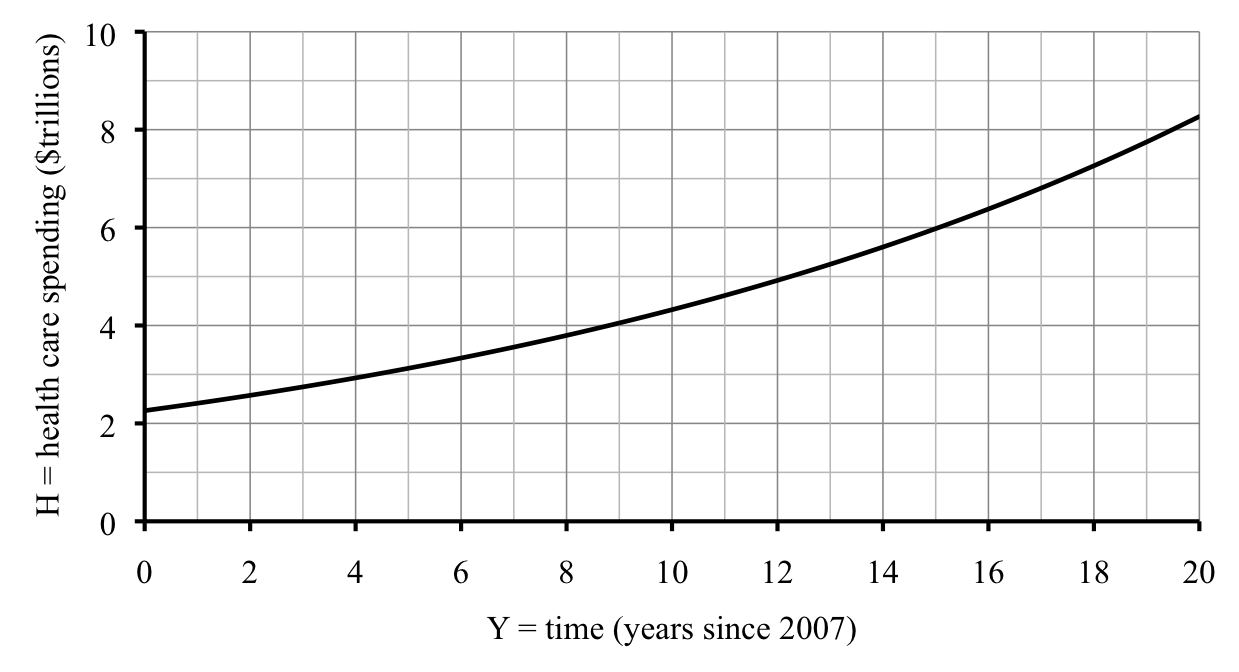
\includegraphics [width = 6in] {healthcarecosts.png}}
\end{center}
Can you see that the graph curves slightly?  It's not a line.  That's because this function isn't linear.
 
Look back at our equation $$H = 2.26\ast 1.067^{Y}$$
This type of equation is called an \textbf{exponential equation} because the independent variable is in the exponent.  
Any exponential equation fits this template.

\bigskip
 \framebox{
 \begin{minipage}[c]{.85\textwidth}  
~ \bigskip \\  \textsc{Exponential equation template:} \quad $\text{dep} = \text{start} \ast \text{growth factor} ^ {\text{indep}}$\\ ~ \vspace{.01in} %VSPACE
\end{minipage}
}
\bigskip

Notice our two variables are in our equation and there are two constants. Each constant has its own meaning.  The first constant is 2.26 and it is measured in trillions of dollars.  It is the amount spent on health care in the starting year of 2007.  In our standard form we refer to this quantity as the \textbf{starting value} (or \textbf{start} for short).  As with linear equations, it's official name is \textbf{intercept} and it's the value where the curve crosses the vertical axis on the graph.

The second constant is the growth factor 1.067, and is the decimal equivalent of the 106.7\%.  The growth factor for an exponential equation is similar to the slope of a linear equation because both tell us how fast the function is increasing.  But the slope measures the rate of change -- how much is added at each step, while the growth factor corresponds to the percent increase.  Another way to say that is linear functions correspond to situations where we are adding the same amount each time and exponential functions correspond to situations where we are adding the same percentage each time (or, equivalently, multiplying by the same amount each time).

Sometimes the graph of an exponential equation looks a lot like a  line, especially if you only plot a few points.  So, be sure to plot five or more points to see the curve in the graph of an exponential equation. 

%\section{A first look at exponential equations}

 \begin{center}
\line(1,0){300} %\line(1,0){250}
\end{center}

\section*{Homework}

\noindent \textbf{Start by doing Practice exercises \#1-4 in the workbook.}

\bigskip

\noindent \textbf{Do you know \ldots}

\begin{itemize}  
\item How to find the growth factor if you know the percent increase?    
\item How to calculate percent increase in one step?   
\item What makes a function exponential?   
\item The template for an exponential equation? \emph{Ask your instructor if you need to remember the template or if it will be provided during the exam.} 
\item Where the starting value and growth factor appear in the template for an exponential equation?   
\item What the graph of an exponential function looks like? 
 \item[~] \textbf{If you're not sure, work the rest of exercises and then return to these questions.  Or, ask your instructor or a classmate for help.} 
\end{itemize}

\subsection*{Exercises}

\begin{enumerate} 
\setcounter{enumi}{4}

\item Mai's salary was \$78,000 before she got a 6\% raise.  Now the economy was not doing as well and she got only a 1.5\% raise this year.
\begin{enumerate}
\item What was her salary after the second raise?
\item Her colleague Tom\'a\u s started with a salary of \$78,000 but did not get a raise the first year like Mai did.  What percentage raise would Tom\'a\u s need now in order to have the same final salary as Mai?
\item Would Mai's salary have been the more than, less than, or the same as now if she had received the 1.5\% raise first and then the 6\% raise?
\item Which order would you rather have:  6\% then 1.5\% or 1.5\% then 6\%?  Why?
\end{enumerate}

\item The number of school children in the district from a single parent household has been on the rise.  In one district there were 1,290 children from single parent households in 2010 and that number was expected to increase about 3\% per year.

\hfill \emph{Story also appears in 3.4 and 5.3 Exercises}
\begin{enumerate}
\item Calculate the annual growth factor.
\item How many children from single parent households are expected in that district by 2015?
\item Name the variables and write an equation relating them.
\item Make a table showing the number of school children in the district from a single parent household in 2010, 2015, 2020, and 2030.
\item Graph the function.  
\end{enumerate}

\item Um Archivo data consultant group reported earnings of \$42.7 billion in 2012.  At that time executives projected 17\% increase in earnings annually. 

 \hfill \emph{Story also appears in 5.1 Exercises}
\begin{enumerate}
\item Name the variables and find an equation relating them.
\item According to your equation, what would Um Archivo's earnings be in 2020.
\item If Um Archivo reports earnings of \$78.1 billion in 2020, would you say the projected rate of 17\% was too high or too low?  Explain.
\item Draw a graph showing how Um Archivo's profits are expected to increase.
\end{enumerate}  

\item In 2005, poultry production was 78 million tons estimated to be growing at a rate of around 1.6\% per year.   
\hfill \begin{footnotesize} Source:  Worldwatch Institute \end{footnotesize} 

 \hfill \emph{Story also appears in 3.4 Exercises}
\begin{enumerate}
\item Write an equation showing how poultry production is expected to rise. Don't forget to name the variables.
\item Make a table showing the production in 2005, 2010, 2020, and 2050 (at least according to the equation.)
\end{enumerate} 

\item Back in January 2008, e-book sales were averaging \$5.1 million per month and were increasing approximately 6.3\% per month.  (We are ignoring seasonal variation in this problem.)
%By 2010, that had jumped to around \$263.0 million.  
\hfill \begin{footnotesize} Source:  ReadWriteWeb \end{footnotesize} 

\begin{enumerate}
\item Name the variables including units.
\item Calculate the monthly growth factor.
\item Write an exponential equation illustrating this dependence.  
\item By January 2010, monthly sales averaged 21.9 million.  How does that compare to your equation's estimate?
\item What does your equation project for average monthly ebook sales in January 2014?
\end{enumerate}

\end{enumerate}